\documentclass[letterpaper,10pt]{article}

\usepackage{enumitem}
\usepackage{titling}
\usepackage{listings,listings-rust}
\usepackage{url}
\usepackage{soul}
\usepackage{hyperref}
\usepackage{setspace}
\usepackage{subfig}
\usepackage{sectsty}
\usepackage{pdfpages}
\usepackage{colortbl}
\usepackage{multirow}
\usepackage{multicol}
\usepackage{relsize}
\usepackage{amsmath}
\usepackage{wasysym}
\usepackage{fancyvrb}
\usepackage[yyyymmdd]{datetime}
\usepackage{amsmath,amssymb,amsthm,graphicx,xspace}
\usepackage[titlenotnumbered,noend,noline]{algorithm2e}
\usepackage[compact]{titlesec}
\usepackage{XCharter}
\usepackage[T1]{fontenc}
\usepackage[scaled]{beramono}
\usepackage[normalem]{ulem}
\usepackage{booktabs}
\usepackage{tikz}
\usetikzlibrary{arrows.meta,automata,shapes,trees,matrix,chains,scopes,positioning,calc,decorations.pathreplacing}
\tikzstyle{block} = [rectangle, draw, fill=blue!20, 
    text width=2.5em, text centered, rounded corners, minimum height=2em]
\tikzstyle{bw} = [rectangle, draw, fill=blue!20, 
    text width=4em, text centered, rounded corners, minimum height=2em]

\definecolor{namerow}{cmyk}{.40,.40,.40,.40}
\definecolor{namecol}{cmyk}{.40,.40,.40,.40}
\renewcommand{\dateseparator}{-}

\let\LaTeXtitle\title
\renewcommand{\title}[1]{\LaTeXtitle{\textsf{#1}}}

\lstset{basicstyle=\footnotesize\ttfamily,breaklines=true}

\newcommand{\CPP}{C\nolinebreak\hspace{-.05em}\raisebox{.4ex}{\tiny\bf +}\nolinebreak\hspace{-.10em}\raisebox{.4ex}{\tiny\bf +}}
\def\CPP{{C\nolinebreak[4]\hspace{-.05em}\raisebox{.4ex}{\tiny\bf ++}}}

\newcommand{\handout}[5]{
  \noindent
  \begin{center}
  \framebox{
    \vbox{
      \hbox to 5.78in { {\bf ECE459: Programming for Performance } \hfill #2 }
      \vspace{4mm}
      \hbox to 5.78in { {\Large \hfill #4  \hfill} }
      \vspace{2mm}
      \hbox to 5.78in { {\em #3 \hfill \today} }
    }
  }
  \end{center}
  \vspace*{4mm}
}

\newcommand{\lecture}[3]{\handout{#1}{#2}{#3}{Lecture#1}}
\newcommand{\tuple}[1]{\ensuremath{\left\langle #1 \right\rangle}\xspace}

\addtolength{\oddsidemargin}{-1.000in}
\addtolength{\evensidemargin}{-0.500in}
\addtolength{\textwidth}{2.0in}
\addtolength{\topmargin}{-1.000in}
\addtolength{\textheight}{1.75in}
\addtolength{\parskip}{\baselineskip}
\setlength{\parindent}{0in}
\renewcommand{\baselinestretch}{1.5}
\newcommand{\term}{Winter 2020}

\singlespace


\begin{document}

\lecture{24 --- Profiling}{\term}{Jeff Zarnett \& Patrick Lam}

\section*{Profiling}

Think back to the beginning of the course when we did a quiz on what operations are fast and what operations are not. The important takeaway was not that we needed to focus on how to micro-optimize this abstraction or that hash function, but that our intuition about what is fast and what is slow is often wrong. Not just at a macro level, but at a micro level. You may be able to narrow down that this computation of $x$ is slow, but if you examine it carefully... what parts of it are slow?

If you don't use tools, then you end up guessing. You just make some assumptions about what you think is likely to be slow and try to change it. You've probably heard the famous quotation before, but here it is in its full form:

\begin{quote}
\textit{Programmers waste enormous amounts of time thinking about, or worrying about, the speed of noncritical parts of their programs, and these attempts at efficiency actually have a strong negative impact when debugging and maintenance are considered. We should forget about small efficiencies, say about 97\% of the time: premature optimization is the root of all evil. Yet we should not pass up our opportunities in that critical 3\%.}
\end{quote}
	\hfill -- Donald Knuth

So going about this blindly is probably a waste of time. You might be fortunate and optimize a slow part\footnote{There is a saying that even a blind squirrel sometimes finds a nut.} but we should really follow one of my favourite rules: ``don't guess, measure!''\footnote{Now I am certain you are sick of hearing that.} So, to make your programs or systems fast, you need to find out what is currently slow and improve it (duh!). Up until now in the course it's mostly been about ``let's speed this up'', but we did not take much time to decide what we should speed up (though you maybe did this on your assignment 2...?).

The general idea is, collect some data on what parts of the code are taking up the majority of the time. This can be broken down into looking at what functions get called, or how long functions take, or what's using memory...

There is always the ``informal'' way of doing this; it sort of works but it's not exactly the best plan. You probably know that when developing a program you can ``debug'' it without using any tools (e.g., \texttt{gdb}) by inserting a lot of print statements to the console or the log file. So when you enter function \texttt{foo} you print a nice little line on the console that say something like ``entering function foo'', associated with a timestamp and then when you're ready to return, a corresponding print function that says ``exiting'' appears, also with a timestamp.

This approach kind of works, and I've used it myself to figure out what blocks of a single large function are taking a long time (updating exchange rates... yeah). But this approach is not necessarily a good one.  It's an example of ``invasive'' profiling -- we are going in and changing the source code of the program in question -- to add instrumentation (log/debug statements). Plus we have to do a lot of manual accounting. Assuming your program is fast and goes through functions quickly and often, trying to put the pieces together manually is hopeless. It worked in that one example because the single function itself was running in the half hour range and I could see that the save operation was taking twelve minutes. Not kidding. 

(Also like debugging, if you get to be a wizard you can maybe do it by code inspection, but that technique of speculative execution inside your head is a lot harder to apply to performance problems than it is to debugging.)

So we should all agree, we want to use tools and do this in a methodical way.

Now that we agree on that, let's think about how profiling tools work\:

\begin{itemize}
\item sampling-based (traditional): every so often (e.g. 100ms for gprof), query the
system state; or,
\item instrumentation-based, or probe-based/predicate-based
  (traditionally too expensive): query system state under certain
  conditions; like conditional breakpoints.
\end{itemize}
We'll talk about both per-process profiling and system-wide profiling.

If you need your system to run fast, you need to start profiling
and benchmarking as soon as you can run the system. Benefits:
\begin{itemize}
\item establishes a baseline performance for the system;
\item allows you to measure impacts of changes and further system development;
\item allows you to re-design the system before it's too late;
\item avoids the need for ``perf spray'' to make the system faster, since
that spray is often made of ``unobtainium''\footnote{\url{http://en.wikipedia.org/wiki/Unobtainium}}.
\end{itemize}

\paragraph{Tips for Leveraging Profiling.}
When writing large software projects:
  \begin{itemize}
    \item First, write clear and concise code. \\
      Don't do any premature optimizations---focus on correctness.
    \item Profile to get a baseline of your performance:
      \begin{itemize}
        \item allows you to easily track any performance changes;
        \item allows you to re-design your program before it's too late.
      \end{itemize}
  \end{itemize}
Focus your optimization efforts on the code that matters.

Look for abnormalities; in particular, you're looking for
deviations from the following rules:
\begin{itemize}
\item time is spent in the right part of the system/program;
\item time is not spent in error-handling, noncritical code, or exceptional cases; and
\item time is not unnecessarily spent in the operating system.
\end{itemize}
For instance, ``why is {\tt ps} taking up all my cycles?'';
see page 34 of ~\cite{300ps}.

\paragraph{Development vs. production.}
You can always profile your systems in development, but that might not
help with complexities in production. (You want separate dev and
production systems, of course!) We'll talk a bit about DTrace, which
is one way of profiling a production system. The constraints on profiling 
production systems are that the profiling must not affect the system's
performance or reliability.

\section*{Userspace per-process profiling}
Sometimes---or, in this course, often---you can get away with
investigating just one process and get useful results about that
process's behaviour.  We'll first talk about {\tt gprof}, the GNU
profiler
tool\footnote{\url{http://sourceware.org/binutils/docs/gprof/}}, and
then continue with other tools.

{\tt gprof} does sampling-based profiling for single processes: it
requests that the operating system interrupt the process being
profiled at regular time intervals and figures out which procedure is
currently running. It also adds a bit of instrumentation to collect
information about which procedures call other procedures.

\paragraph{``Flat'' profile.} The obvious thing to do with the
profile information is to just print it out. You get a list of
procedures called and the amount of time spent in each of these 
procedures.

The general limitation is that procedures that don't run for
long enough won't show up in the profile. (There's a caveat: if
the function was compiled for profiling, then it will show up
anyway, but you won't find out about how long it executed for).

\paragraph{``Call graph''.} {\tt gprof} can also print out 
its version of a call graph, which shows the amount of time that
either a function runs (as in the ``flat'' profile) as well as the
amount of time that the callees of the function run.  Another term for
such a call graph is a ``dynamic call graph'', since it tracks the
dynamic behaviour of the program.  Using the {\tt gprof} call graph,
you can find out who is responsible for calling the functions that
take a long time.

\paragraph{Limitations of {\tt gprof}.} Beyond the usual limitations
of a process-oriented profiler, {\tt gprof} also suffers limitations
from running completely in user-space. That is, it has no access to
information about system calls, including time spent doing I/O.
It also doesn't know anything about the CPU's built-in counters
(e.g. cache miss counts, etc). Like the other profilers, it causes
overhead when it's running, but the overhead isn't too large.

\section*{{\tt gprof} usage guide}
We'll give some details about using {\tt gprof}. First,
use the {\tt -pg} flag with {\tt clang} when compiling and linking.
(It's currently broken in gcc, unless you give {\tt -no-pie}.)
Next, run your program as you normally would.
 Your program will now create {\tt gmon.out}.

Use gprof to interpret the results: {\tt gprof <executable>}.

\paragraph*{Example.} Consider a program with 100 million calls 
to two math functions.

\begin{tabular}{ll}
\begin{minipage}{.5\textwidth}
\begin{lstlisting}[language=C,basicstyle=\scriptsize]
int main() {
    int i,x1=10,y1=3,r1=0;
    float x2=10,y2=3,r2=0;

    for(i=0;i<100000000;i++) {
        r1 += int_math(x1,y1);
        r2 += float_math(y2,y2);
    }
}

int int_math(int x, int y){
    int r1;
    r1=int_power(x,y);
    r1=int_math_helper(x,y);
    return r1;
}

int int_math_helper(int x, int y){
    int r1;
    r1=x/y*int_power(y,x)/int_power(x,y);
    return r1;
}

int int_power(int x, int y){
    int i, r;
    r=x;
    for(i=1;i<y;i++){
        r=r*x;
    }
    return r;
}
\end{lstlisting}
\end{minipage}
\begin{minipage}{0.5\textwidth}
\begin{lstlisting}[language=C]
float float_math(float x, float y) {
    float r1;
    r1=float_power(x,y);
    r1=float_math_helper(x,y);
    return r1;
}

float float_math_helper(float x, float y) {
    float r1;
    r1=x/y*float_power(y,x)/float_power(x,y);
    return r1;
}

float float_power(float x, float y){
    float i, r;
    r=x;
    for(i=1;i<y;i++) {
        r=r*x;
    }
    return r;
}
  \end{lstlisting}
\end{minipage}
\end{tabular}

Looking at the code, we have no idea what takes longer.
One might guess that floating point math takes longer. This is admittedly a
silly example, but it works well to illustrate our point.

\paragraph{Flat Profile Example.}
    When we run the program and look at the flat profile, we see:

  \begin{lstlisting}
          Flat profile:

          Each sample counts as 0.01 seconds.
            %   cumulative   self              self     total           
           time   seconds   seconds    calls  ns/call  ns/call  name    
           32.58      4.69     4.69 300000000    15.64    15.64  int_power
           30.55      9.09     4.40 300000000    14.66    14.66  float_power
           16.95     11.53     2.44 100000000    24.41    55.68  int_math_helper
           11.43     13.18     1.65 100000000    16.46    45.78  float_math_helper
            4.05     13.76     0.58 100000000     5.84    77.16  int_math
            3.01     14.19     0.43 100000000     4.33    64.78  float_math
            2.10     14.50     0.30                             main
  \end{lstlisting}

 There is one function per line. Here are what the columns mean:
  \begin{itemize}
    \item {\bf \% time:} the percent of the total execution time in this function.
    \item {\bf self:} seconds in this function.
    \item {\bf cumulative:} sum of this function's time + any above it in table.
    \item {\bf calls:} number of times this function was called.
    \item {\bf self ns/call:} just self nanoseconds / calls.
    \item {\bf total ns/call:} mean function execution time, including
       calls the function makes.
  \end{itemize}

\paragraph{Call Graph Example.}
After the flat profile gives you a feel for which functions are costly, you
      can get a better story from the call graph.

  \begin{lstlisting}
          index % time    self  children    called     name
                                                           <spontaneous>
          [1]    100.0    0.30   14.19                 main [1]
                          0.58    7.13 100000000/100000000     int_math [2]
                          0.43    6.04 100000000/100000000     float_math [3]
          -----------------------------------------------
                          0.58    7.13 100000000/100000000     main [1]
          [2]     53.2    0.58    7.13 100000000         int_math [2]
                          2.44    3.13 100000000/100000000     int_math_helper [4]
                          1.56    0.00 100000000/300000000     int_power [5]
          -----------------------------------------------
                          0.43    6.04 100000000/100000000     main [1]
          [3]     44.7    0.43    6.04 100000000         float_math [3]
                          1.65    2.93 100000000/100000000     float_math_helper [6]
                          1.47    0.00 100000000/300000000     float_power [7]
          -----------------------------------------------
                          2.44    3.13 100000000/100000000     int_math [2]
          [4]     38.4    2.44    3.13 100000000         int_math_helper [4]
                          3.13    0.00 200000000/300000000     int_power [5]
          -----------------------------------------------
                          1.56    0.00 100000000/300000000     int_math [2]
                          3.13    0.00 200000000/300000000     int_math_helper [4]
          [5]     32.4    4.69    0.00 300000000         int_power [5]
          -----------------------------------------------
                          1.65    2.93 100000000/100000000     float_math [3]
          [6]     31.6    1.65    2.93 100000000         float_math_helper [6]
                          2.93    0.00 200000000/300000000     float_power [7]
          -----------------------------------------------
                          1.47    0.00 100000000/300000000     float_math [3]
                          2.93    0.00 200000000/300000000     float_math_helper [6]
          [7]     30.3    4.40    0.00 300000000         float_power [7]
  \end{lstlisting}

To interpret the call graph, note that the line with the index [N] is the \emph{primary line},
or the current function being considered.
\begin{itemize}
    \item Lines above the primary line are the functions which called this function.
    \item Lines below the primary line are the functions which were called by this function
      (children).
\end{itemize}

For the primary line, the columns mean:
  \begin{itemize}  
    \item {\bf time:} total percentage of time spent in this function and its
      children.
    \item {\bf self:} same as in flat profile.
    \item {\bf children:} time spent in all calls made by the function;
      \begin{itemize}
        \item should be equal to self + children of all functions below.
      \end{itemize}
  \end{itemize}

For callers (functions above the primary line):
  \begin{itemize}
    \item {\bf self:} time spent in primary function, when called from current
      function.
    \item {\bf children:} time spent in primary function's children, when
      called from current function.
    \item {\bf called:} number of times primary function was called from current
      function / number of nonrecursive calls to primary function.
  \end{itemize}

For callees (functions below the primary line):
  \begin{itemize}  
    \item {\bf self:} time spent in current function when called from primary.
    \item {\bf children:} time spent in current function's children calls when
      called from primary.
      \begin{itemize}
        \item self + children is an estimate of time spent in current function
          when called from primary function.
      \end{itemize}
    \item {\bf called:} number of times current function was called from primary
      function / number of nonrecursive calls to current function.
  \end{itemize}

Based on this information, we can now see where most of the time comes
from, and pinpoint any locations that make unexpected calls, etc.
This example isn't too exciting; we could simplify the math and optimize the
program that way.

\section*{Introduction to gperftools}
Next, we'll talk about the Google Performance Tools. 
\begin{center}
\url{http://google-perftools.googlecode.com/svn/trunk/doc/cpuprofile.html}
\end{center}
They include:
      \begin{itemize}
        \item a CPU profiler
        \item a heap profiler
        \item a heap checker; and 
        \item a faster (multithreaded) {\tt malloc}.
      \end{itemize}

We'll mostly use the CPU profiler. Characteristics include:
      \begin{itemize}
        \item  supposedly works for
multithreaded programs;
        \item purely statistical sampling;
        \item no recompilation required (typically benefit from re-linking); and
        \item better output, including built-in graphical output.
      \end{itemize}

You can use the profiler without any recompilation. But this is not recommended;
you'll get worse data. Use {\tt LD\_PRELOAD}, which changes the dynamic libraries that
an executable uses.

  \begin{lstlisting}[basicstyle=\scriptsize]
  % LD_PRELOAD="/usr/lib/libprofiler.so" CPUPROFILE=test.prof ./test
  \end{lstlisting}

The other (more-recommended) option is to link to the profiler with {\tt -lprofiler}.

Both options read the {\tt CPUPROFILE} environment variable, which
specifies where profiling data goes.

You can use the profiling library directly as well:
\begin{lstlisting}[basicstyle=\scriptsize]
          #include <gperftools/profiler.h>
\end{lstlisting}
Then, bracket code you want profiled with:
\begin{lstlisting}[basicstyle=\scriptsize]
          ProfilerStart()
          // ...
          ProfilerStop()
\end{lstlisting}
    
You can change the sampling frequency with the {\tt CPUPROFILE\_FREQUENCY} environment variable
(default value 100 interrupts/second).

\paragraph{{\tt pprof} usage.} {\tt pprof} is like {\tt gprof} for Google Perf Tools. It
analyzes profiling results. Here are some usage examples.
  \begin{lstlisting}[basicstyle=\scriptsize]
          % pprof test test.prof
              Enters "interactive" mode
          % pprof --text test test.prof
              Outputs one line per procedure
          % pprof --gv test test.prof
               Displays annotated call-graph via 'gv'
          % pprof --gv --focus=Mutex test test.prof
              Restricts to code paths including a .*Mutex.* entry
          % pprof --gv --focus=Mutex --ignore=string test test.prof
              Code paths including Mutex but not string
          % pprof --list=getdir test test.prof
              (Per-line) annotated source listing for getdir()
          % pprof --disasm=getdir test test.prof
              (Per-PC) annotated disassembly for getdir()
  \end{lstlisting}

Can also output {\tt dot}, {\tt ps}, {\tt pdf} or {\tt gif} instead of {\tt gv}.

\paragraph{{\tt pprof} text output.}
This is similar to the flat profile in {\tt gprof}.

  \begin{lstlisting}[basicstyle=\scriptsize]
          jon@riker examples master % pprof --text test test.prof 
          Using local file test.
          Using local file test.prof.
          Removing killpg from all stack traces.
          Total: 300 samples
                95  31.7%  31.7%      102  34.0% int_power
                58  19.3%  51.0%       58  19.3% float_power
                51  17.0%  68.0%       96  32.0% float_math_helper
                50  16.7%  84.7%      137  45.7% int_math_helper
                18   6.0%  90.7%      131  43.7% float_math
                14   4.7%  95.3%      159  53.0% int_math
                14   4.7% 100.0%      300 100.0% main
                 0   0.0% 100.0%      300 100.0% __libc_start_main
                 0   0.0% 100.0%      300 100.0% _start
  \end{lstlisting}

Columns, from left to right, denote:
\begin{itemize}
\item  Number of samples in this function.
\item  Percentage of samples in this function (same as {\bf time} in {\tt gprof}).
\item  Percentage of checks in the functions printed so far (equivalent to {\bf cumulative}, but in \%).
\item     Number of checks in this function and its callees.
\item     Percentage of checks in this function and its callees.
\item    Function name.
\end{itemize}

\paragraph{Graphical Output.} Google Perf Tools can also produce graphical output:

\begin{center}
    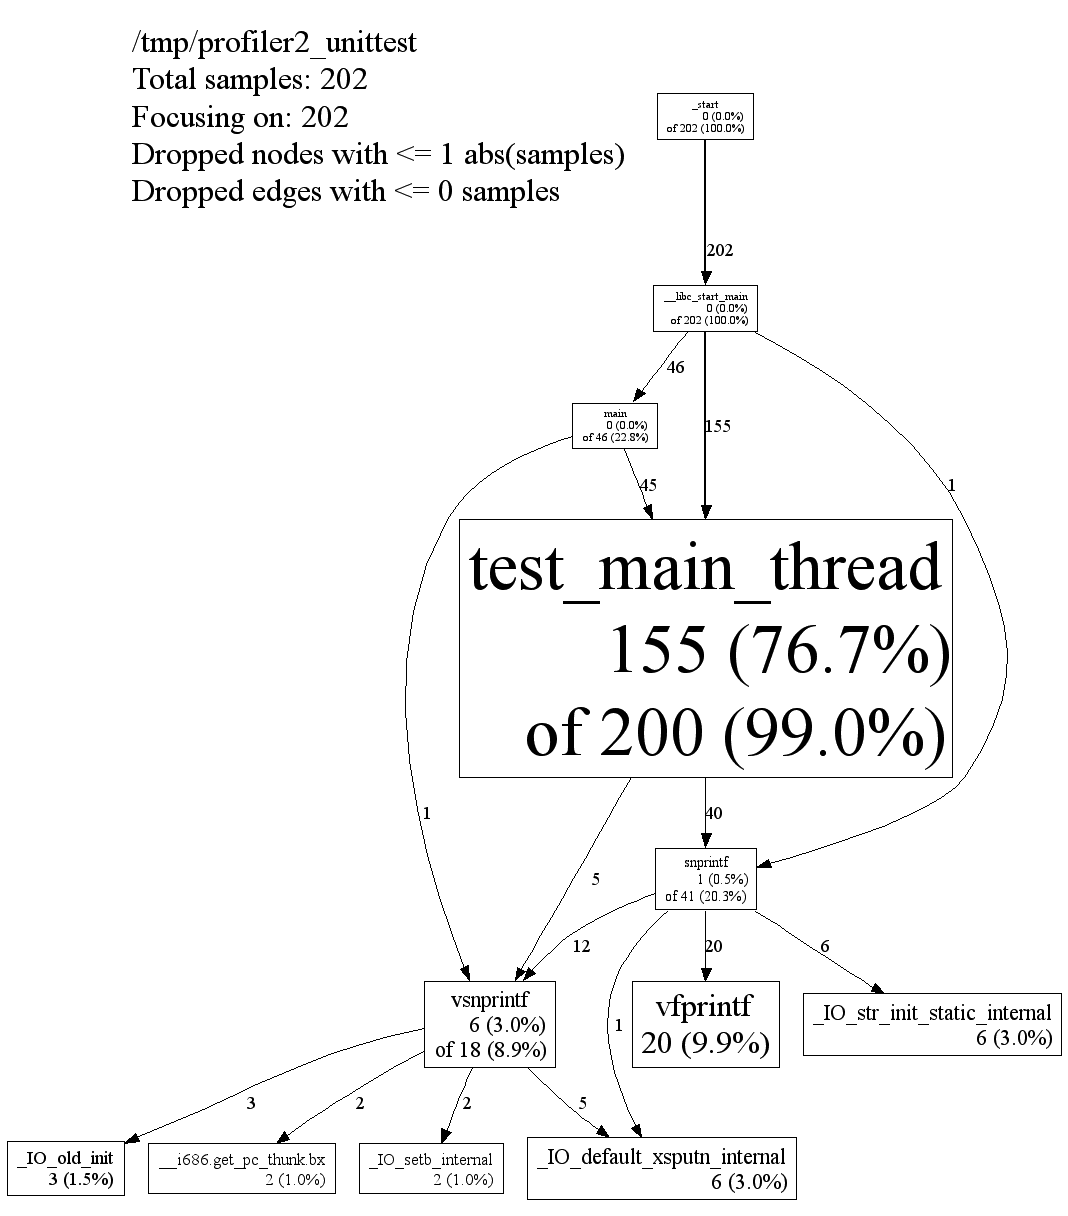
\includegraphics[scale=0.3]{images/pprof-test-big.png}
\end{center}

This shows the same numbers as the text output. This particular graphical example is on a different program than the text output, and that's why they look different. Directed edges denote function calls.
Note: 
\[ \mbox{\# of samples in callees} = \mbox{\# in ``this function + callees''} - \mbox{\# in ``this function''}.\]

For example, in {\tt float\_math\_helper}, we have ``51 (local) of 96 (cumulative)''.
Here,
\[ 96 - 51 = 45 \mbox{ (callees)}. \]
      \begin{itemize}
        \item callee {\tt int\_power} = 7 (bogus)
        \item callee {\tt float\_power} = 38
        \item callees total = 45
      \end{itemize}

Note that the call graph is not exact.
In fact, it shows many bogus relations which clearly don't exist.
For instance, we know that there are no cross-calls between {\tt int} and {\tt float} functions.

As with {\tt gprof}, optimizations will change the
      graph.\

You'll probably want to look at the text profile first, then use the
      {\tt --focus} flag to look at individual functions.


\bibliographystyle{alphaurl}
\bibliography{459}


\end{document}
